\section{Caracterizando os Horários com Maior Valor de Tráfego}

Nesta seção, os horários com maior valor médio das taxas de upload e download para cada tipo de dispositivo, Smart TV e Chromecast, foram analisados seguindo os passos descritos.

\subsection{Passo 1: Seleção dos Horários}

A partir dos gráficos de médias por hora apresentados Figura~\ref{fig:estatisticas_por_hora}, os horários com maior valor médio para cada taxa e dispositivo foram identificados:
\begin{itemize}
    \item \textbf{Smart TV:}
        \begin{itemize}
            \item dataset 1: composto pelo horário com maior média de upload (20:00).
            \item dataset 2: composto pelo horário com maior média de download (20:00).
        \end{itemize}
    \item \textbf{Chromecast:}
        \begin{itemize}
            \item dataset 3: composto pelo horário com maior média de upload (22:00).
            \item dataset 4: composto pelo horário com maior média de download (23:00).
        \end{itemize}
\end{itemize}

\subsection{Passo 2: Histogramas dos Dados}

Histogramas foram gerados para cada um dos 4 datasets criados no Passo 1. O método de Sturges (Equação~\ref{eq:sturges}) foi utilizado para determinar o número adequado de bins, obtendo-se os seguintes valores:

\begin{itemize}
    \item \textbf{Dataset 1}(Smart TV - Upload)\textbf{:}  19 bins
    \item \textbf{Dataset 2}(Smart TV - Download)\textbf{:}  19 bins
    \item \textbf{Dataset 3}(Chromecast - Upload)\textbf{:}  20 bins
    \item \textbf{Dataset 4}(Chromecast - Download)\textbf{:}  20 bins
\end{itemize}

Esses histogramas destacam os padrões de distribuição das taxas de upload e download para os horários selecionados, conforme ilustrado na Figura~\ref{fig:histogramas_horarios}.

\begin{figure}[H]
    \centering
    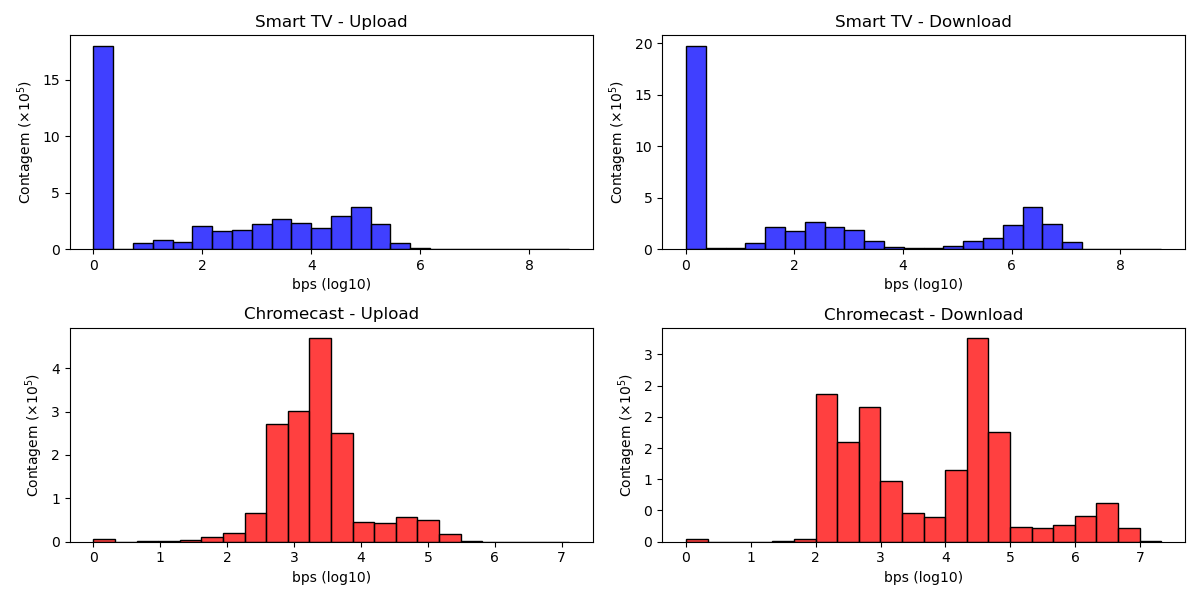
\includegraphics[width=0.8\textwidth]{../caracterizando os horários/histogramas.png}
    \caption{Histogramas das taxas de upload e download para os horários selecionados.}
    \label{fig:histogramas_horarios}
\end{figure}

\subsection{Passo 3: Estimativa de Parâmetros via MLE}

Os parâmetros das distribuições Gaussiana e Gamma foram estimados utilizando o método de Máxima Verossimilhança (\textit{Maximum Likelihood Estimation} - MLE) para os quatro conjuntos de dados. Esses valores foram aplicados na modelagem das distribuições, permitindo uma análise comparativa com os dados observados.

O MLE consiste em determinar os parâmetros que maximizam a função de verossimilhança, que mede a probabilidade dos dados observados para um conjunto de parâmetros. Para simplificar os cálculos, o logaritmo da verossimilhança (\textit{log-likelihood}) é utilizado. A derivada da \textit{log-likelihood} é igualada a zero para encontrar os estimadores de máxima verossimilhança dos parâmetros.

As funções de densidade de probabilidade para as distribuições Gaussiana e Gamma são definidas como:

\begin{itemize}
    \item \textbf{Gaussiana:}
    \begin{equation}
        f(x) = \frac{1}{\sigma \sqrt{2\pi}} e^{-\frac{(x - \mu)^2}{2\sigma^2}}
    \end{equation}
    onde \(\mu\) é a média e \(\sigma^2\) é a variância da distribuição.
    
    \item \textbf{Gamma:}
    \begin{equation}
        f(x) = \frac{\beta^\alpha x^{\alpha - 1} e^{-x/\beta}}{\Gamma(\alpha)}
    \end{equation}
    onde \(\alpha\) é o parâmetro de forma, \(\beta\) é o parâmetro de escala, e \(\Gamma(\alpha)\) é a função Gamma, definida como \(\int_0^\infty x^{\alpha - 1} e^{-x} dx\).
\end{itemize}

Para a distribuição Gaussiana, as estimativas dos parâmetros são obtidas de forma direta:

\begin{equation}
    \hat{\mu} = \frac{1}{n} \sum_{i=1}^{n} x_i, \quad \hat{\sigma}^2 = \frac{1}{n} \sum_{i=1}^{n} (x_i - \hat{\mu})^2
\end{equation}

No caso da distribuição Gamma, a estimação dos parâmetros \(\alpha\) (forma) e \(\beta\) (escala) pelo MLE não possui soluções analíticas simples e geralmente requer métodos numéricos iterativos. O parâmetro \(\alpha\) é frequentemente estimado utilizando o método de Newton-Raphson aplicado à função de log-verossimilhança, enquanto \(\beta\) pode ser estimado a partir de \(\alpha\) e da média amostral \(\bar{x}\) \cite{minka2002estimating}:

\begin{equation}
    \hat{\beta} = \frac{\bar{x}}{\hat{\alpha}}
\end{equation}

Para realizar essas estimativas, foi utilizado o método `gamma.fit` da biblioteca `scipy.stats` do Python. Este método aplica o MLE de forma eficiente, empregando algoritmos de otimização numérica para determinar os parâmetros que melhor se ajustam aos dados observados. A função `gamma.fit` retorna estimativas para os parâmetros de forma (\(\alpha\)) e escala (\(\beta\)) da distribuição Gamma, facilitando a modelagem estatística dos dados.

Os resultados das estimativas de parâmetros via MLE para as distribuições Gaussiana e Gamma são apresentados na Tabela~\ref{tab:resultados_mle}.

\begin{table}[H]
    \centering
    \caption{Resultados das estimativas de parâmetros via MLE}
    \label{tab:resultados_mle}
    \begin{tabular}{|c|c|c|c|c|}
        \hline
        \textbf{Dataset} & \textbf{$\hat{\mu}$} & \textbf{$\hat{\sigma}^2$} & \textbf{$\hat{\alpha}$} & \textbf{$\hat{\beta}$} \\ 
        \hline
        Dataset 1 (Smart TV - Upload) & 3.1243 & 3.1687 & 0.4937 & 6.3308 \\ 
        \hline
        Dataset 2 (Smart TV - Download) & 3.3961 & 6.2013 & 0.4078 & 8.3307 \\ 
        \hline
        Dataset 3 (Chromecast - Upload) & 3.5215 & 0.5957 & 8.7654 & 0.4019 \\ 
        \hline
        Dataset 4 (Chromecast - Download) & 4.0527 & 2.1594 & 4.7261 & 0.8577 \\ 
        \hline
    \end{tabular}
\end{table}

Além disso, as \textit{log-likelihoods} e \textit{likelihoods} para as distribuições Gaussiana e Gamma são apresentadas na Tabela~\ref{tab:likelihoods}. As \textit{log-likelihoods} foram calculadas primeiro, para evitar erros de \textit{underflow} ao calcular as \textit{likelihoods}, substituindo a multiplicação de valores muito pequenos pela soma de seus logaritmos naturais.
\begin{table}[H]
    \centering
    \caption{Likelihoods ($L$) e Log-likelihoods ($log[L]$) para os Datasets}
    \label{tab:likelihoods}
    \begin{tabular}{|c|c|c|c|c|}
        \hline
        \textbf{Dataset} & \textbf{$log[L]$ Gaussiana} & \textbf{$L$ Gaussiana} & \textbf{$log[L]$ Gamma} & \textbf{$L$ Gamma} \\ 
        \hline
        Dataset 1 (Smart TV - Upload) & -424282 & 0.0 & -406884 & 0.0 \\ 
        \hline
        Dataset 2 (Smart TV - Download) & -495658 & 0.0 & -387106 & 0.0 \\ 
        \hline
        Dataset 3 (Chromecast - Upload) & -89011 & 0.0 & -119219 & 0.0 \\ 
        \hline
        Dataset 4 (Chromecast - Download) & -129603 & 0.0 & -141373 & 0.0 \\ 
        \hline
    \end{tabular}
\end{table}


\subsection{Passo 4: Gráficos de Densidade}

Gráficos contendo o histograma dos dados e as funções de densidade Gaussiana e Gamma, parametrizadas pelos valores obtidos no Passo 3, foram gerados e estão disponíveis na Figura~\ref{fig:histogramas_pdf}. Esses gráficos possibilitam uma comparação visual da aderência de cada distribuição aos dados reais.

\begin{figure}[H]
    \centering
    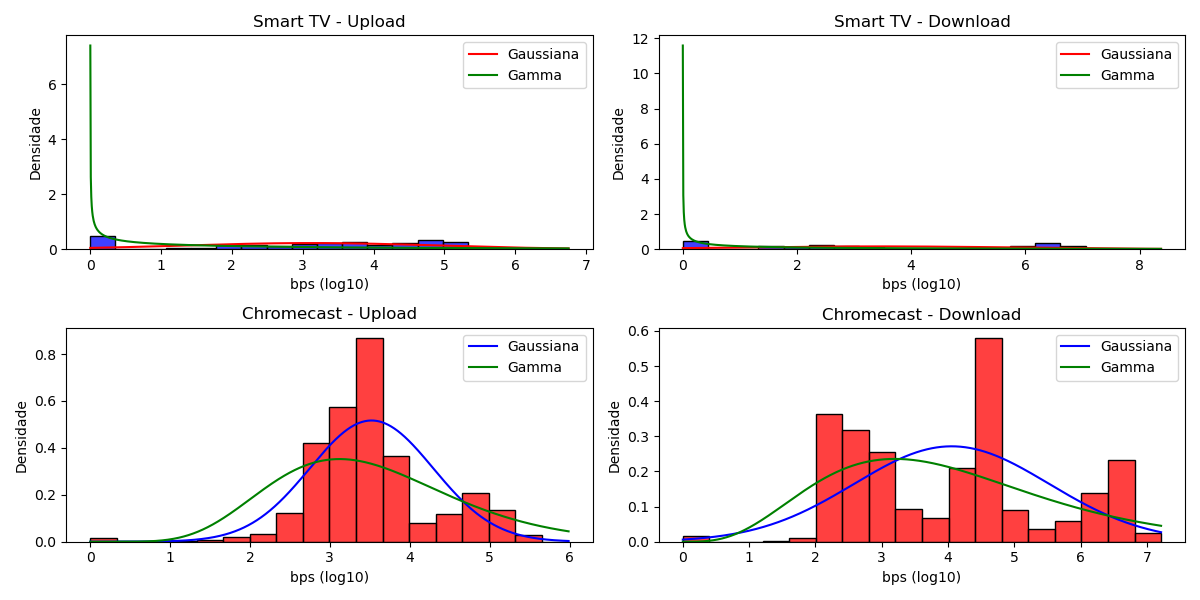
\includegraphics[width=0.8\textwidth]{../caracterizando os horários/histogramas_pdf.png}
    \caption{Histogramas dos dados e funções de densidade parametrizadas para as distribuições Gaussiana e Gamma.}
    \label{fig:histogramas_pdf}
\end{figure}

Observando a figura, é possível notar que nenhuma das distribuições propostas (Gaussiana e Gamma) se ajusta bem aos dados observados. A distribuição Gamma inclusive explode para valores muito baixos dos dados referentes a Smart TV. 

Voltando na figura \ref{fig:histogramas_horarios}, é possível observar que os dados não seguem uma distribuição normal e nem gamma, o que pode ser um dos motivos para a má aderência das distribuições propostas. Uma sugestão seria utilizar uma mistura de distribuições para representar os dados, da seguinte forma:

\begin{itemize}
    \item \textbf{Dataset 1 (Smart TV - Upload):} Mistura de uma Gaussiana e uma Gamma.
    \item \textbf{Dataset 2 (Smart TV - Download):} Mistura de três Gaussianas.
    \item \textbf{Dataset 3 (Chromecast - Upload):} Mistura de duas Gaussianas.
    \item \textbf{Dataset 4 (Chromecast - Download):} Mistura de uma Gaussiana e duas Gammas.
\end{itemize}



\subsection{Passo 5: Probability Plots}

\textit{Probability Plots} foram criados para comparar os dados reais com as distribuições parametrizadas (Gaussiana e Gamma). No total, 8 gráficos foram gerados, permitindo avaliar a adequação das distribuições propostas aos dados.

\subsection{Passo 6: QQ Plots}

\textit{QQ Plots} foram produzidos para comparar os datasets de upload e download entre os dispositivos (Smart TV e Chromecast). A interpolação linear foi utilizada para alinhar os quantis dos datasets de tamanhos diferentes. Esses gráficos permitem a análise das similaridades entre os padrões de tráfego dos dispositivos.

\subsection{Análise dos Resultados}

Com base nos resultados, as seguintes questões foram avaliadas:
\begin{enumerate}
    \item \textbf{Quais foram os horários escolhidos para cada dataset?}
    \item \textbf{O que foi observado a partir dos histogramas?}
    \item \textbf{Quais diferenças e/ou similaridades foram identificadas entre os datasets 1, 2, 3 e 4?}
    \item \textbf{É possível caracterizar os datasets por uma variável aleatória conhecida na literatura? Se não, por quê?}
    \item \textbf{O que foi observado a partir dos gráficos \textit{QQ Plot} e \textit{Probability Plot}?}
\end{enumerate}
% As conclusões são apresentadas em termos de suas implicações para o gerenciamento da rede e o entendimento dos padrões de tráfego para Smart TVs e Chromecasts.
